% Standalone source for the photon transfer / detector-model box diagram.
% Build: make figures/calibration_boxes_detector_model.pdf
% (Or: cd figures/src && pdflatex -interaction=nonstopmode -halt-on-error \
%      -jobname=calibration_boxes_detector_model -output-directory=.. \
%      to-make-calibration-boxes-detector-model.tex)
%
% Text is left at the document's default \normalsize so that, once placed
% in the two-column figure* in sections/2_lsstcam.tex, labels read at the
% same size as the body text.
\documentclass[tikz, border=4pt]{standalone}
\usepackage{times}
\usetikzlibrary{positioning, arrows.meta, calc, fit, shapes.geometric}

\tikzset{
  comp/.style={draw, thick, rounded corners=4pt, align=center,
               minimum height=1.5cm, inner sep=3pt, fill=white},
  effect/.style={draw, dashed, rounded corners=4pt, align=center,
                 inner sep=3pt, font=\itshape, fill=white},
  grouptitle/.style={align=left, font=\bfseries\normalsize},
  gaincap/.style={align=center, font=\normalsize},
  sigflow/.style={-{Latex[length=2.2mm,width=1.6mm]}, thick},
  effflow/.style={-{Latex[length=1.9mm,width=1.3mm]}, dashed},
}

\begin{document}
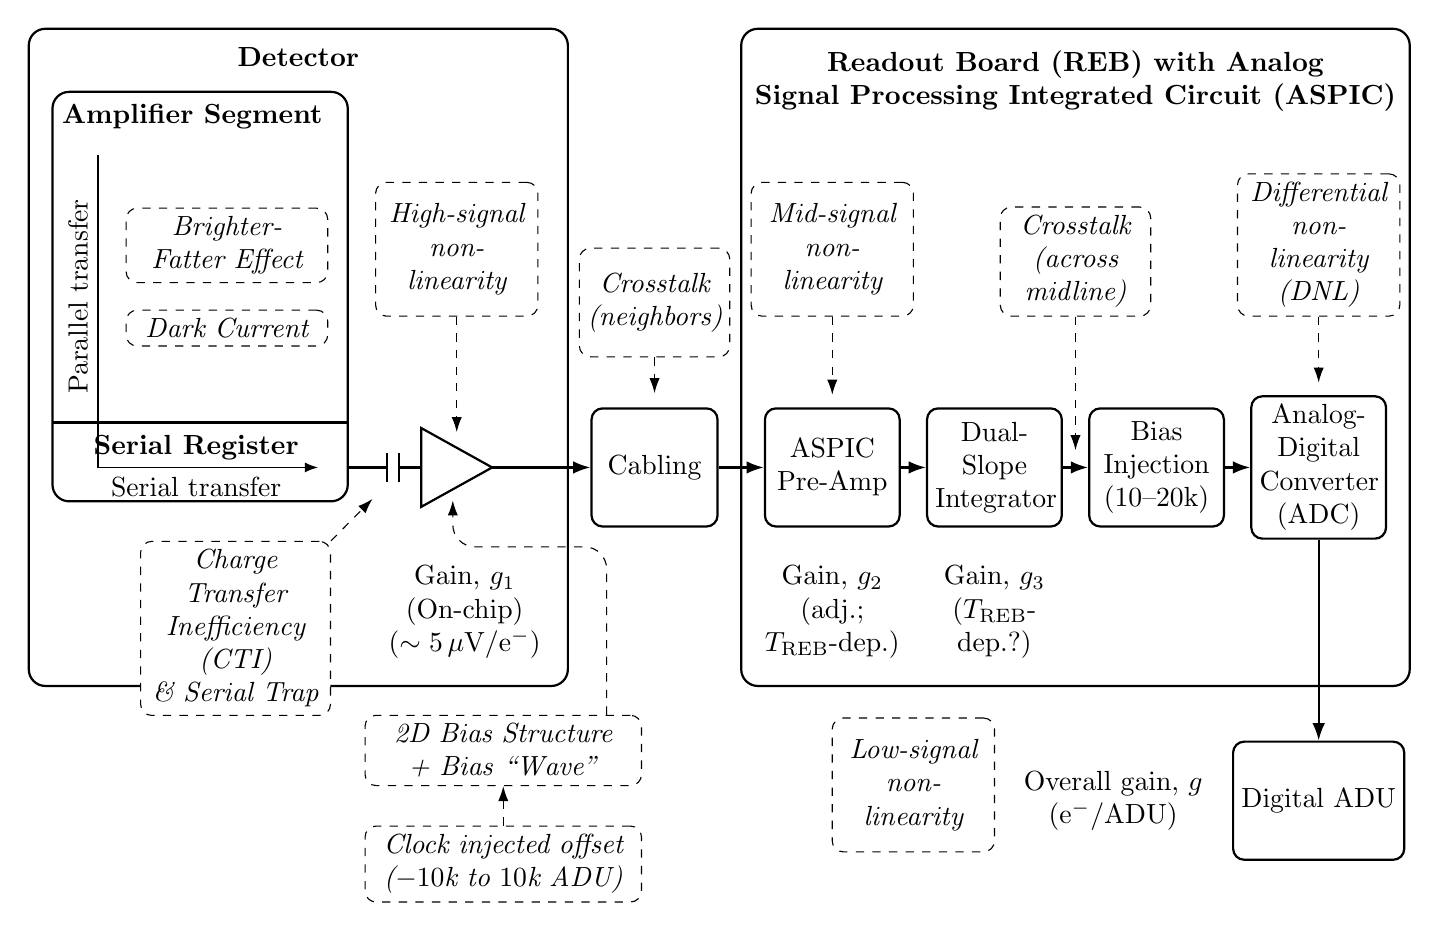
\begin{tikzpicture}[>=Latex, font=\normalsize]

% ================= amplifier segment (solid box) =================
\node[draw, thick, rounded corners=6pt, minimum width=3.75cm, minimum height=5.2cm] (amp) at (0,0) {};
\node[font=\normalsize\bfseries] at (-.1,2.28) {Amplifier Segment};

% -- L-shaped charge-transfer path: parallel transfer, then serial transfer/register --
\draw[semithick] (-1.3,1.8) -- (-1.3,-2.17) -- (1.4,-2.17);
\draw[semithick,-{Latex[length=1.7mm]}] (1.0,-2.17) -- (1.5,-2.17);
\draw[thick] (-1.875,-1.6) -- (1.875,-1.6);

% \draw[thick, double distance=1.1pt] (-0.85,-0.9) -- (0.5,-0.9);
\node[font=\normalsize, rotate=90] at (-1.55,0.0) {Parallel transfer};
\node[font=\normalsize] at (-0.05,-1.92) {\textbf{Serial Register}};
\node[font=\normalsize] at (-0.05,-2.42) {Serial transfer};

% ================= coupling capacitor + preamplifier triangle =================
% Exit the amplifier on the serial-transfer line (y=-2.17), not at mid-height.
\coordinate (ampout) at (amp.east |- 0,-2.17);
\coordinate (capL) at ($(ampout)+(0.48,0)$);
\coordinate (capR) at ($(ampout)+(0.64,0)$);
\draw[thick] (ampout) -- (capL);
\draw[thick] ($(capL)+(0,-0.18)$) -- ($(capL)+(0,0.18)$);
\draw[thick] ($(capR)+(0,-0.18)$) -- ($(capR)+(0,0.18)$);
\coordinate (preamp-in) at ($(capR)+(0.28,0)$);
\draw[thick] (capR) -- (preamp-in);
\coordinate (preamp-tip) at ($(preamp-in)+(0.90,0)$);
\draw[thick, fill=white] ($(preamp-in)+(0,0.5)$) -- (preamp-tip) -- ($(preamp-in)+(0,-0.5)$) -- cycle;
\node[coordinate] (preamp-top) at ($(preamp-in)+(0,0.5)$) {};
\node[coordinate] (preamp-bot) at ($(preamp-in)+(0,-0.5)$) {};

\coordinate (g1-home) at ($(preamp-in)+(0.55,-1.25)$);
\node[gaincap, text width=2.0cm, opacity=0, text opacity=0] (g1box) at (g1-home) {Gain, $g_1$\\(On-chip)\\($\sim5\,\mu$V/e$^-$)};

% Brighter-Fatter and Dark Current as separate, floating, disconnected boxes.
\node[effect, text width=2.35cm] (bf) at (0.34,0.65) {Brighter-Fatter Effect};
\node[effect, text width=2.35cm] (dc) at (0.34,-0.40) {Dark Current};
% Pin keeps the detector outline where it was when this box sat below the amplifier.
\coordinate (bf-pin) at (0,-3.828);

% ================= Detector dotted enclosure =================
% Headroom above the amplifier keeps the Detector title clear of that box.
\node[fit=(amp)(bf-pin)(preamp-tip)(g1box), inner sep=0pt] (detfit) {};
\coordinate (det-nw) at ($(detfit.north west)+(-0.28,0.78)$);
\coordinate (det-east) at ($(detfit.south east)+(0.18,0)$);

% ================= rest of the signal chain =================
% ASPIC stays put (1.1cm + cabling width + 1.25cm from the preamp tip).
% Cabling is placed later, centered between the detector and REB outlines.
\node[comp, minimum width=1.7cm, text width=1.5cm, right=3.45cm of preamp-tip] (aspic) {ASPIC\\Pre-Amp};

\node[comp, minimum width=1.7cm, text width=1.5cm, right=0.32cm of aspic] (dsi) {Dual-Slope\\Integrator};
\draw[sigflow] (aspic.east) -- (dsi.west);

\node[comp, minimum width=1.7cm, text width=1.5cm, right=0.32cm of dsi] (bias) {Bias\\Injection\\($10$--$20$k)};
\draw[sigflow] (dsi.east) -- (bias.west);

\node[comp, minimum width=1.7cm, text width=1.5cm, right=0.32cm of bias] (adc) {Analog-\\Digital\\Converter (ADC)};
\draw[sigflow] (bias.east) -- (adc.west);

\node[comp, minimum width=1.6cm, below=2.55cm of adc] (adu) {Digital ADU};
\draw[sigflow] (adc.south) -- (adu.north);
\node[gaincap, anchor=east] at ($(adu.west)+(-0.25,0)$) {Overall gain, $g$\\(e$^-$/ADU)};

% ================= REB dotted enclosure (fit around all four REB boxes) =================
\node[fit=(aspic)(dsi)(bias)(adc), inner sep=0pt] (rebfit) {};
% Top edge stays at its previous height (boxes dropped 2.17cm onto y=-2.17;
% the old north offset was 1.25). The south edge follows the lowered boxes.
\coordinate (reb-nw) at ([xshift=-0.28cm]rebfit.north west |- det-nw);
\coordinate (reb-se) at ($(rebfit.south east)+(0.28,-1.85)$);
\draw[rounded corners=6pt, thick] (reb-nw) rectangle (reb-se);

% Detector bottom matches the REB bottom. On-chip gain drops by the same amount.
\coordinate (det-se) at (det-east |- reb-se);
\draw[rounded corners=6pt, thick] (det-nw) rectangle (det-se);
\node[grouptitle, align=center, anchor=north] at ($(det-nw)!0.5!(det-se |- det-nw)+(0,-0.12)$) {Detector};
\path let \p1=($(detfit.south)+(0,-0.22)$), \p2=(reb-se), \n1={\y2-\y1} in
  node[gaincap, text width=2.0cm] (g1) at ($(g1-home)+(0,\n1)$) {Gain, $g_1$\\(On-chip)\\($\sim5\,\mu$V/e$^-$)};
\node[gaincap, text width=2.0cm, anchor=north] (g2) at (aspic |- g1.north) {Gain, $g_2$\\(adj.; $T_{\mathrm{REB}}$-dep.)};
\node[gaincap, text width=2.0cm, anchor=north] (g3) at (dsi |- g1.north) {Gain, $g_3$\\($T_{\mathrm{REB}}$-dep.?)};
\node[grouptitle, align=center, anchor=north] at ($(reb-nw)!0.5!(reb-se |- reb-nw)+(0,-0.15)$)
  {Readout Board (REB) with Analog\\Signal Processing Integrated Circuit (ASPIC)};

\coordinate (cab-x) at ($(det-se)!0.5!(reb-nw)$);
\node[comp, minimum width=1.6cm, anchor=center] (cab)
  at (cab-x |- preamp-tip) {Cabling};
\draw[sigflow] (preamp-tip) -- (cab.west);
\draw[sigflow] (cab.east) -- (aspic.west);

% ================= effect annotations: above the chain =================
% Same size and the same bottom edge. High-signal arrow drops straight down.
\coordinate (tri-mid) at ($(preamp-in)!0.5!(preamp-tip)$);
\coordinate (nl-row) at ($(aspic.north)+(0,1.15)$);
\node[effect, minimum width=2.05cm, minimum height=1.7cm, text width=1.85cm, anchor=south] (hsnl)
  at (tri-mid |- nl-row) {High-signal\\non-linearity};
\draw[effflow] (hsnl.south) -- ($(hsnl.south |- tri-mid)+(0,0.45)$);

% Same size as crosstalk (across midline), and on the same row.
\node[effect, minimum width=1.9cm, minimum height=1.38cm, text width=1.7cm, anchor=south] (xtn)
  at ($(det-se)!0.5!(reb-nw)$ |- nl-row)
  {Crosstalk\\(neighbors)};
\draw[effflow] (xtn.south) -- ($(cab.north)+(0,0.18)$);

% Sits where the g2 label was, above the ASPIC, and stops short of that box.
\node[effect, minimum width=2.05cm, minimum height=1.7cm, text width=1.85cm, anchor=south] (midnl)
  at (aspic.north |- nl-row) {Mid-signal\\non-linearity};
\draw[effflow] (midnl.south) -- ($(aspic.north)+(0,0.16)$);

\node[effect, minimum width=2.05cm, minimum height=1.7cm, text width=1.85cm, anchor=south] (dnl)
  at (adc.north |- nl-row) {Differential\\non-linearity (DNL)};
\draw[effflow] (dnl.south) -- ($(adc.north)+(0,0.16)$);

% ================= effect annotations: below the chain =================
\node[effect, minimum width=2.4cm, text width=2.2cm] (cti) at ($(amp.south)+(0.45,-1.6)$) {Charge Transfer\\Inefficiency (CTI)\\ \& Serial Trap};
\draw[effflow] (cti.north east) -- ($(capL)+(-0.18,-0.40)$);

\node[effect, minimum width=3.5cm, text width=3.3cm] (bias2d) at ($(amp.south)+(3.85,-3.15)$) {2D Bias Structure\\+ Bias ``Wave''};
\coordinate (bias-out) at ($(bias2d.north east)+(-0.45,0)$);
\coordinate (tri-below) at ($(preamp-in)+(0.40,-0.42)$);
\coordinate (bias-run) at ($(g1.north)+(0,0.12)$);
\draw[effflow, rounded corners=8pt] (bias-out)
  -- (bias-out |- bias-run)
  -- (tri-below |- bias-run)
  -- (tri-below);

\node[effect, minimum width=3.5cm, text width=3.3cm, below=0.5cm of bias2d] (clk) {Clock injected offset\\($-10$k to $10$k ADU)};
\draw[effflow] (clk.north) -- (bias2d.south);

\coordinate (aspic-dsi-mid) at ($(aspic.east)!0.5!(dsi.west)$);
\node[effect, minimum width=2.05cm, minimum height=1.7cm, text width=1.85cm, anchor=north] (lownl)
  at ($(aspic-dsi-mid |- reb-se)+(0,-0.4)$) {Low-signal\\non-linearity};

\coordinate (dsi-bias-mid) at ($(dsi.east)!0.5!(bias.west)$);
\node[effect, minimum width=1.9cm, minimum height=1.38cm, text width=1.7cm, anchor=south] (xtm)
  at (dsi-bias-mid |- midnl.south) {Crosstalk\\(across midline)};
  % Change minimum width and text width to widen the box
  [effect, minimum width=2.6cm, text width=2.3cm, anchor=south]
  at (dsi-bias-mid |- midnl.south) {Crosstalk\\(across midline)};
\draw[effflow] (xtm.south) -- ($(dsi-bias-mid)+(0,0.22)$);

\end{tikzpicture}
\end{document}
